\begin{figure}[htbp]
\centering
\captionsetup{
  justification=raggedright,
  labelsep=none,
  singlelinecheck=false,
  labelformat=boldlabel,
}
\caption[Cumulative net return: ML Ensemble vs. human managers.]{\footnotesize \textbf{: Cumulative net return: ML Ensemble vs. human managers.} Cumulative wealth index (compounded net monthly returns) over the out-of-sample window for the eight ML Ensemble portfolio-construction schemes (net of transaction costs and a 1\% p.a. management fee), FUNDS\_MEAN, FUNDS\_Q75 and IBOV (dotted, to distinguish it from the dashed band). The dashed band shows the 5th--95th percentile of individual fund wealth paths each month across eligible funds, illustrating the dispersion of outcomes underlying the FUNDS\_MEAN average. The cohort holds funds alive at the start of the window; a fund leaves the cohort (and the band) once it stops reporting returns.}
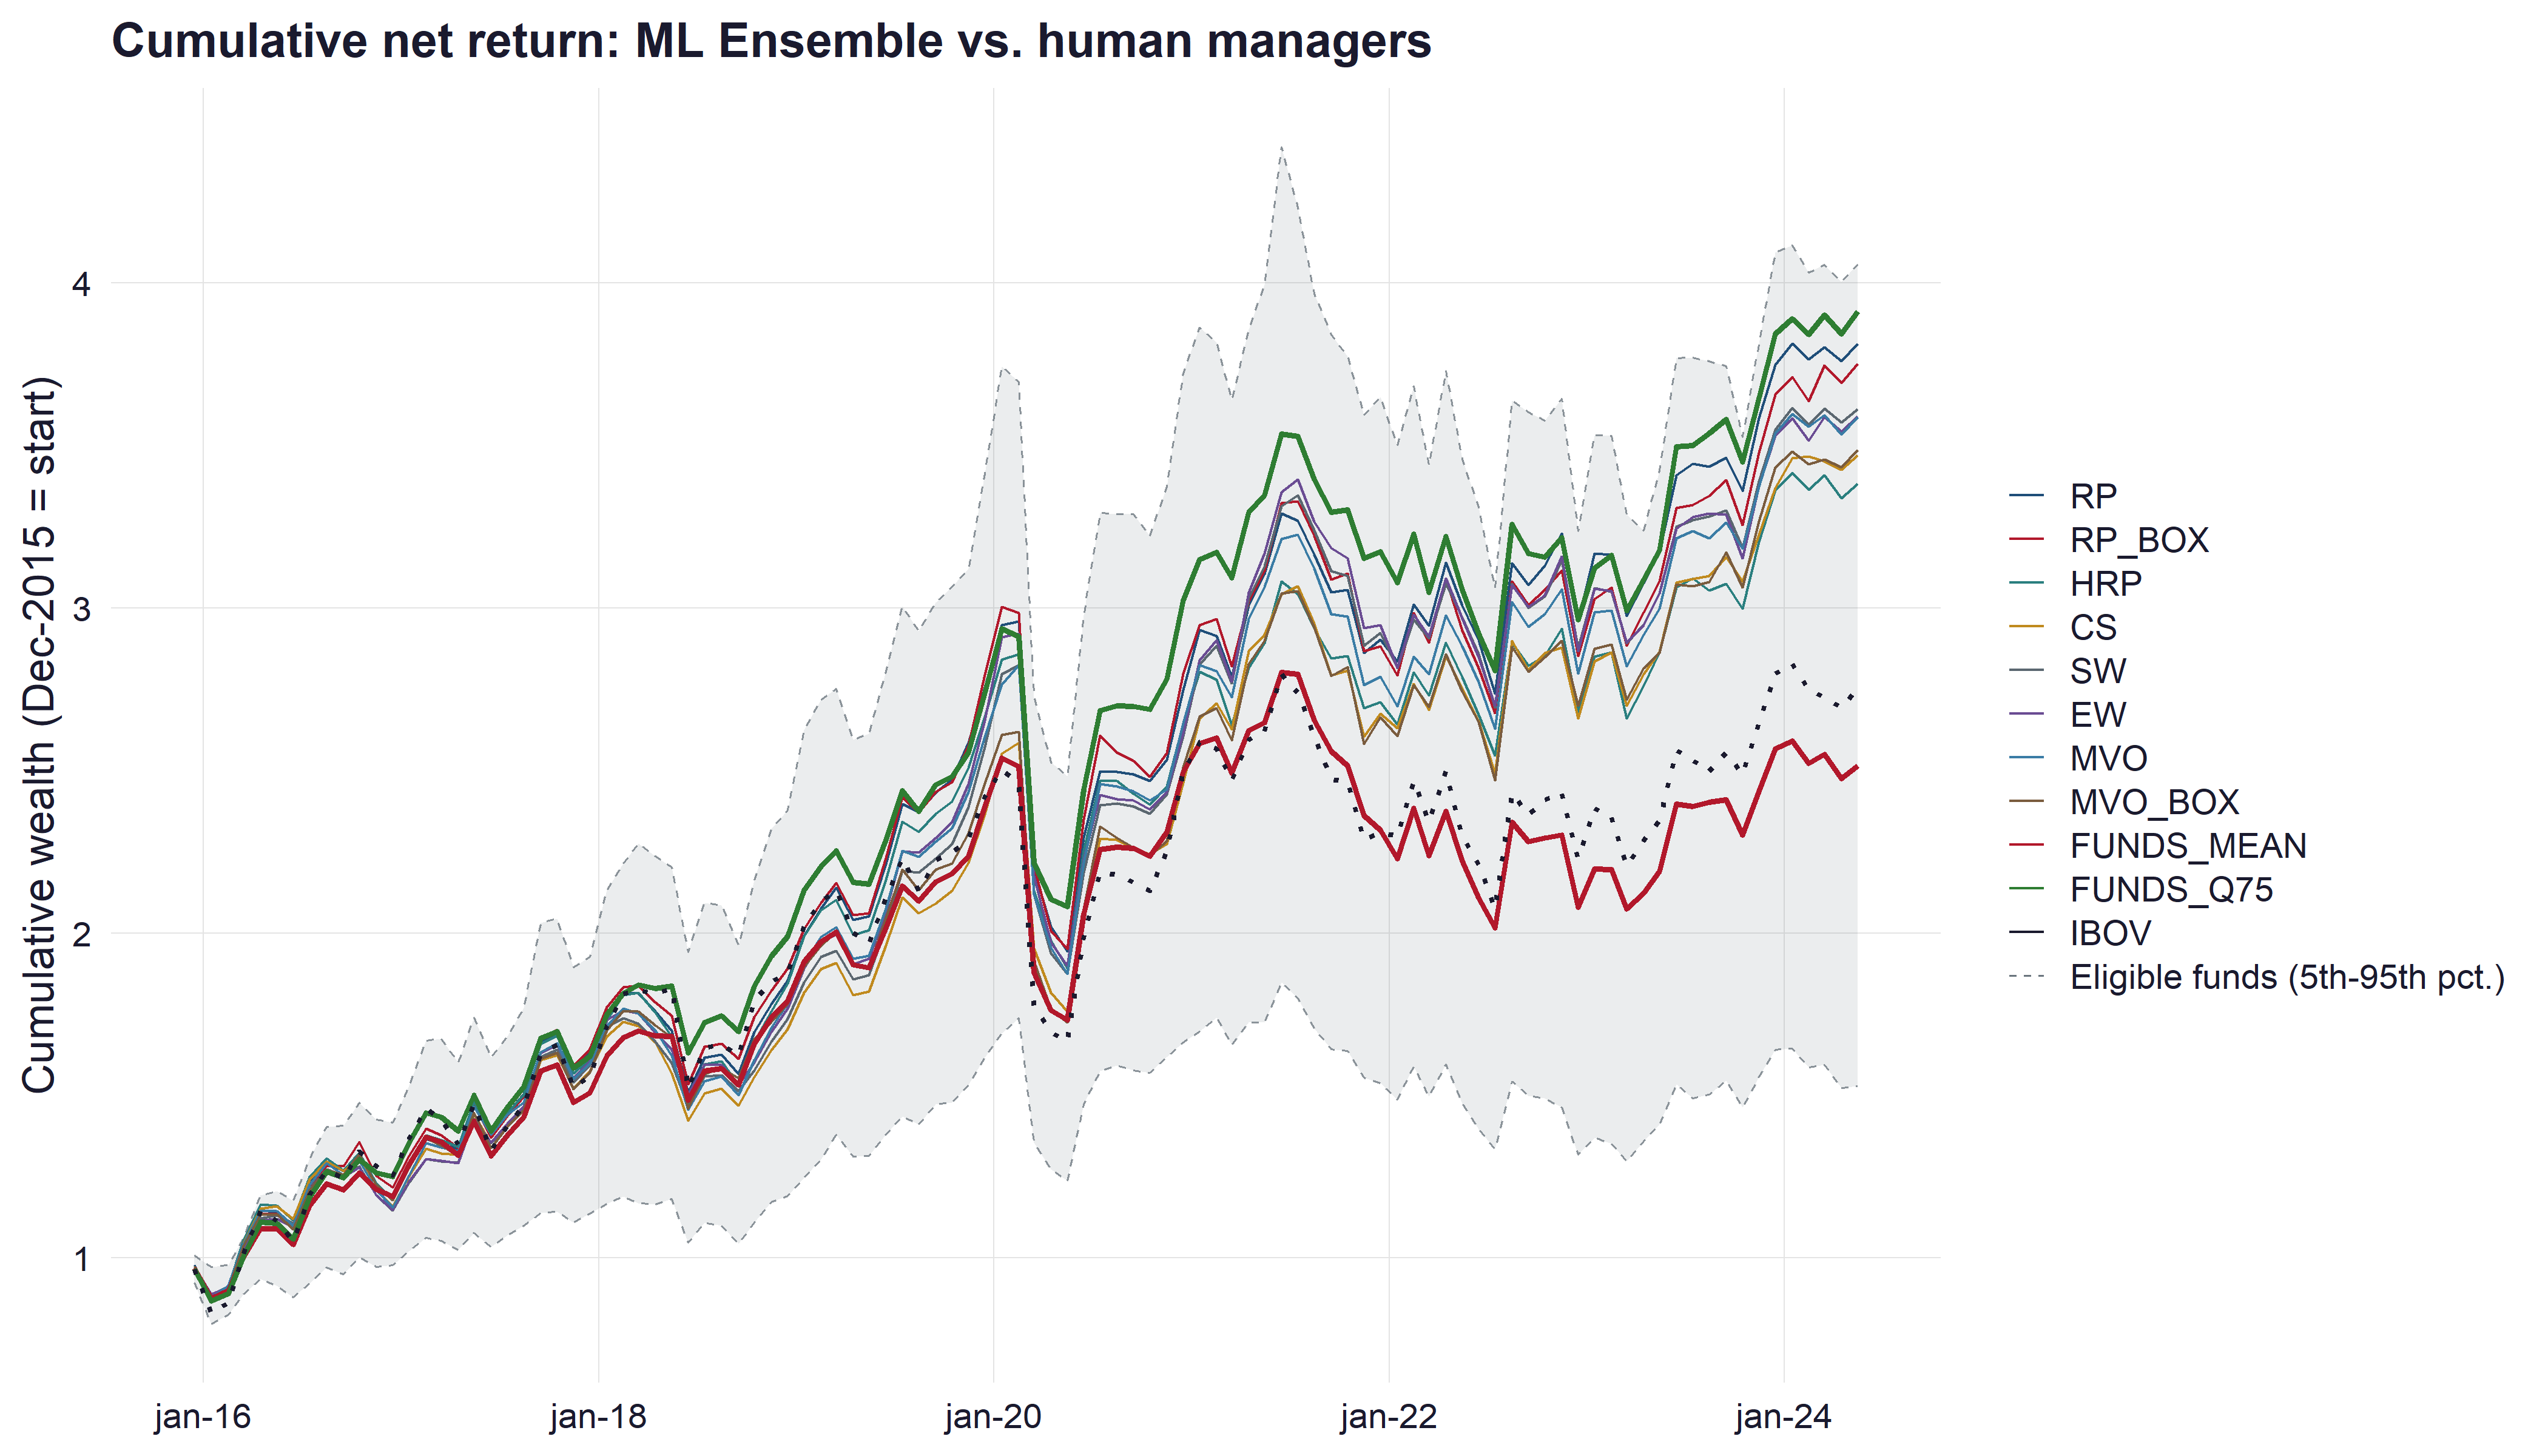
\includegraphics[width=\linewidth]{figures/cumulative_return.png}
\label{fig:cumret}
\end{figure}
